\documentclass[11pt,letterpaper]{article}
\usepackage{listings}
\usepackage{xcolor}
\usepackage{caption}
\usepackage{graphicx}
\usepackage{hyperref}
\usepackage[letterpaper,left=1in,right=1in,top=1in,bottom=1in]{geometry}

% Caption setup
\DeclareCaptionFont{white}{\color{white}}
\DeclareCaptionFormat{listing}{
\parbox{\textwidth}{\colorbox{gray}{\parbox{\textwidth}{#1#2#3}}\vskip=4pt}}
\captionsetup[lstlisting]{format=listing,labelfont=white,textfont=white}

% Indent Paragraphs
\setlength{\parindent}{1cm}

\DeclareGraphicsExtensions{.pdf,.png,.jpg}
\lstset{
	basicstyle=\ttfamily\scriptsize,
	breaklines=true
	frame=lrb,
	xleftmargin=\fboxsep,
	xrightmargin=-\fboxsep
}

\title{Explorations in Parallel and Distributed Sorting Algorithms}
\author{Andrew D. Wong (\texttt{awong16@u.rochester.edu})\\
	Parallel and Distributed Systems\\
	Spring 2013\\
}


\begin{document}
\belowcaptionskip=-10pt
\maketitle

\section{Background}
Sorting, one of computer science classic problems, has been an area of research
since the dawn of computing.  Despite being one of the first algorithms taught
to introductory computer science students, sorting numbers, keys, strings, and
other types of data plays a critical role in nearly all computational tasks.
\par
Research into sorting algorithms was largely conducted on systems with a single
computational unit.  On these systems, a number of sorting algorithms have
achieved performance on the order of $O(n log(n))$ on average.  However, recent
hardware trends and limitations in heat dissipation have increased development
in multi-core often with shared memory.  Additionally, general purpose graphics
processing units and other types of largely parallel processing arrays have been
introduced as coprocessors on devices ranging from systems on a chip to
supercomputers.   As a result, research into parallel and distributed algorithms
has become a major focus in computation theory.  Optimization of sorting
algorithms can be one of the most effective ways to improve a system or
application's performance.  Sorting is heavily used in database systems where
query results may need to be sorted before being returned to the user.
\par
In this paper, I will discuss both comparison and non-comparison based sorting
algorithms and provide results and analysis of the data used in the sorting
algorithms.  Additionally, I will discuss my simplistic distributed sorting
system which I have coined WONG-sort.

\subsection{Issues in Parallel and Distributed Sorting}
There are a number of issues regarding sorting algorithms when attempting to
convert them from a sequential to a parallel context.  Parallelizing algorithms
is complex as the implementation details differ by the algorithms.  Many of
these parallel sorts attempt to take advantage of the data parallelism or the
ability to distribute portions of data to different threads or processes.

\section{Comparison-based Sorts}
The rudimentary sorting algorithm orders an array of numbers either in an
increasing or decreasing fashion.  This is generally done by comparing the
values of two or more numbers then exchanging or swapping the positions of the
numbers through various means.  Unlike non-comparison based sorts, comparison
based sorts allow sorting of all types of data including floating point numbers.
As a result, these are used as general purpose sorting algorithms, however, the
best sorts available have an average case of $O(n log(n))$.
\subsection{Mergesort}
The basic mergesort one of the simplest yet one of the most easy sorts to
parallelize.  The first step in Mergesort is to bisection the array into two
arrays recursively.  Once each array is size of zero or one, the arrays are
merged by comparing the “heads” of the two arrays and selecting the lower value
or non empty value until the two arrays are fully merged into one array.  This
is done recursively until the array is fully sorted.  This achieves an average
case runtime of $O(n logn)$.  One of the issues with merge sort is that a buffer
is required to store the temporarily merged array and thus cannot be completely
done in place.
\par
This sort is implicitly parallel as the first step is to partition the array
into two parts.  Thus one way to parallelize the process is to have a new thread
compute one side of the partition after the bisection.  The merge step can be
completed by having one of the threads finish and the other thread complete the
merging process.  I chose not to implement the parallel version of this sort
because the sequential version proved to be fast enough.

\subsection{Bitonic}
Bitonic sort is an extension on the merge sort algorithm that is often used in
sorting networks.  It makes use of bitonic sequences which are defined as
sequences that are either increasing or decreasing.  The bitonic sort, like the
merge sort, bisections the array and recursively sorts each size as either an
increasing or decreasing sequence.  The base condition, like merge sort is an
array of size one which simply returns.  The merging process uses the fact that
two partitions that are being merged are either increasing and decreasing, or
decreasing and increasing.  As a result, the arrays can be compared starting at
the beginning of the array and each element can be recursively swapped until the
merged array is either in decreasing or increasing order.  Due to the bitonicity
requirement, this sort can only be performed on arrays that are size 2kfor any
k.  As a result of the recursive merging, this sorting algorithm achieves an
average case runtime of $O(n log^2(n))$.
\par
Parallelizing this sort almost identical to the parallelization of the
mergesort.  My implementation additionally uses a data parallel loop and I
utilize the thread’s id to determine which sections of the loop to run. Due to
the bitonic nature of the sort, and the fixed comparison and swaps, this sort
can be performed in place and is a good choice for GPGPUs as it follows the
single instruction multiple data pattern (SIMD).
\par
When testing my implementation of bitonic merge sort, I noticed that a 
significant amount of time was spent in the recursive merge step.  To improve
performance, I modified the algorithm to use a insertion sort when falling below
a certain threshold.  After running some tests, I determined the best threshold
was an array size of 32, as insertion sort provides significant speed up over
bitonic merging.

\subsection{QuickSort}
QuickSort is a well known sorting algorithm that is also easy to parallelize
developed by Tony Hoare that also partitions the input array.  Instead of
bisectioning the array as the above sorts do, QuickSort selects an element in
the array to use as the divider.  All the elements less than the selected
element are place in one partition, all the elements that are larger than the
selected element are placed in another partition.  This is done recursively
until the full array is sorted.  It’s average case sort time is 
$O(n log(n))$ but can have a worse worst case runtime of $O(n^2)$ which is worse
than mergesort.
\par
Althougth I chose not to parallelize this sort, parallelizing this algorithm also is not difficult as it divides the data into
two separate partitions. One of these partitions can be executed on by a new
thread thereby parallelizing the algorithm.   An advanced adaptive
implementation of quicksort, qsort, is used as the default sort in stdlib.h.
\subsection{SampleSort}
SampleSort is a comparison based sort that takes samples across the whole array
then selects n - 1 elements as dividers to partition the elements into n bins.
After being placed in bins, the bins are then sorted using another sort.  I
chose to use my implementation of radix sort as it provided relatively decent
performance across arrays of integers. As the samples are randomly chosen, this
is an example of a randomized parallel sort.
\par
This sort is inherently parallel however there is complexity when using multiple
threads to partition the data.  The threads need to ensure that they do not
“step on each other” when placing elements in a bin when completing the sort
in-place.  A sequential version of this sort would only have one bin and as a
result its is almost completely based off of the helper sort that it uses to
sort the bin. The time complexity of the parallel version of the sort depends on
the helper sort used, but overhead does take $O(\frac{n}{p})$ on average to
place the elements in the bins.   

\section{Non-Comparison Sorts}
One would expect that non-comparison based sorts would not use comparisons
however it is a bit of a misnomer.  Comparison may be used, but comparisons are
generally not used to fully compare an element to another element then order the
element based on the result.  Non-comparison sorts generally use bins or
grouping to continuously sort an array, however these sorts can not be used as
general purpose sorts as they need to be specifically tailored to work on a
particular data type. 
\subsection{Radix Sort} 
Radix sort uses binning to group parts of elements until the array is sorted.
In my particular implementation, I chose to sort integers and examined the each
bit in the integer to use as the binning construct resulting in two groups for
each bit in the integer.  Due to the lack of full comparisons the algorithm
completes in $O(kn)$ for some constant k.
\par
My implementation starts from the steps most significant bit and moves to the
least significant bit and performs the sort in place.  This algorithm can be
parallelized by starting from the least significant bit, and splitting the array
evenly for each thread, then counting the total number of elements that would be
grouped into each bin, then having each thread place their respective elements
into the proper place into the binned array. 

\section{Distributed Sorting}
I also attempted to implement a distributed sort that uses a cluster of
computers to sort an input set of data residing on one machine and utilize the
whole cluster as a distributed sorting network.  After reading previous work on
WIND-sort \cite{data} and psort \cite{psort} I created a basic distributed sort
that transfers data to various slave nodes then uses a sorting algorithm within
each slave to sort the data. Once complete, the data is sent back to the master
which merges the data.
\par
I attempted to follow the implementation described by psort \cite{psort} as it
is currently one of the leaders in distributed sorting benchmarks.  My
implementation called WONG-sort, has a master node that uses a TCP connection
to connect to the slaves, then sends out the data to the appropriate nodes.
The slaves then use sample sort to sort the data, before sending the data back
on the same TCP connection.  The master node then uses a k-way merge to
finalize the sorting process.  The master and slave nodes both use memory maps
tied to files to both simulate an environment that requires an external sort
and simultaneously simplify the processes of mapping memory to a file.

\section{Testing} 
I implemented a driver program that can run the sorts on various arrays of data
and verify the correctness of the sort.  I chose to use two different test
cases: one array was completely random integers, and the other array is an an
array sorted in reverse order.  When testing the program I used array sizes of
$2^{20}$ through $2^{24}$ and used thread numbers from 1, 2, 4, 8, 16, and on niagara1, 32.  These values were chosen because bitonic sort only support arrays of size $2^k$.

The programs work correctly on both the cycle servers and the niagara1.  I
chose to test the parallel sorting algorithms largely on cycle2 which has 2
Intel Xeon X5660s, with 6 cores per CPU and a total of 24 physical threads.
Niagara1 has a UltraSPARC T1 processor with 32 physical threads despite having
only four floating point units.  Due to the fact that the tests were completed
on arrays of integers, the limited number of floating point units did not act
as a major bottleneck. As these are shared machine, I attempted to mitigate
user contention by ensuring that there were no other high priority or CPU
intensive programs running simultaneously.

The distributed sorts were tested on a number of lab machines to simulate 
``commodity hardware''. I used cycle2 as the master that would merge the data
after receiving the computations from all other servers.  These lab computers have Intel i5-2500 processors at 3.30GHz with 6144KB of cache, four cores, and 4 GB of RAM.  The file to be sorted is 512MB and would be equally distributed across all participating nodes.
  
\subsection{Testing Challenges}
One of the major challenges that I encountered when creating the sample tests
and running the driver was the amount of data that could be allocated.  I had
trouble allocating more than 2GB of RAM in user space even though the test
machine  that I was on (cycle2) had more than 24GB gb of RAM and over 20GB
unused.

\section{Results}
\subsection{Sorting Algorithm Comparisons}
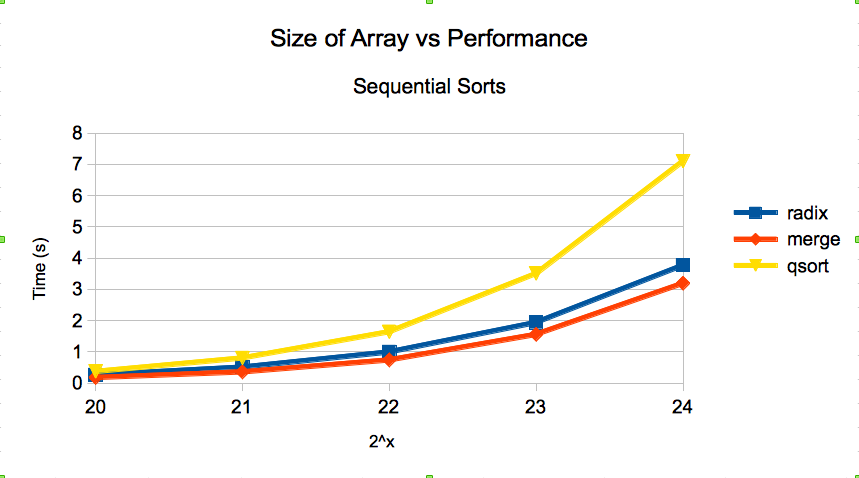
\includegraphics[width=\textwidth]{sequential-performance.png}
\par
It is important to note the performance of some of the sequential sorts available.  Many of these sequential sorts have performance on par with some of the sequential sorts despite the parallel usage of resources.  Merge sort, in particular, is able to outperform the bitonic sort.
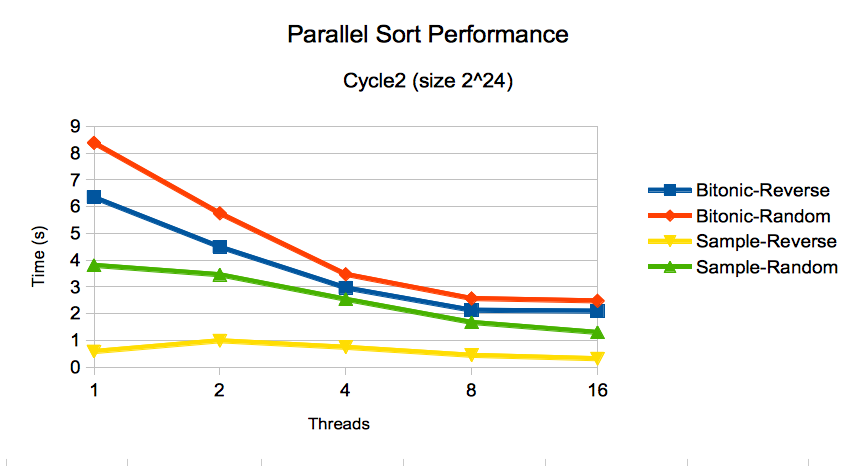
\includegraphics[width=\textwidth]{cycle2-performance.png}
\par When running these tests on cycle2, performance increases dramatically up to four threads but soon levels off after reaching eight threads.\\
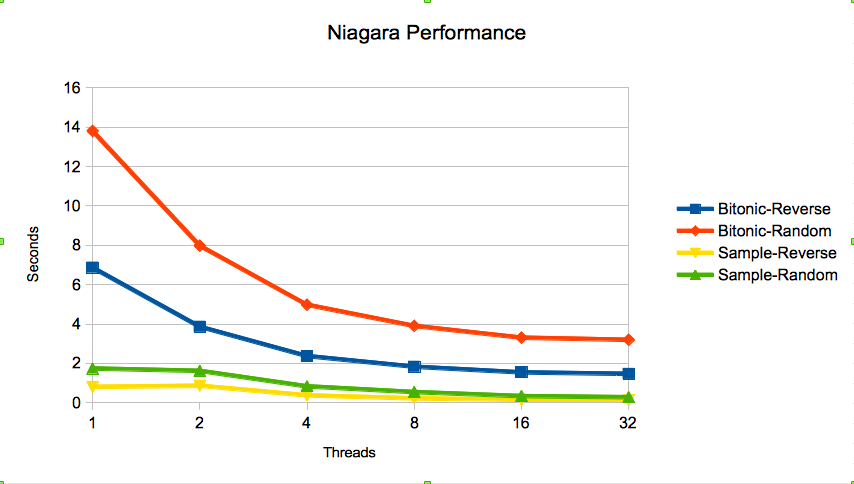
\includegraphics[width=\textwidth]{niagara-performance.png}
\par
On niagara using a size of $2^20$ the bitonic sort improved 4.67 times and the sample sort improved 6.21 times.
\subsection{Distributed Sort (WONG-sort)}
My distributed sorting implementation was performed on a number of Linux nodes
and used cycle2 as the master node.\\
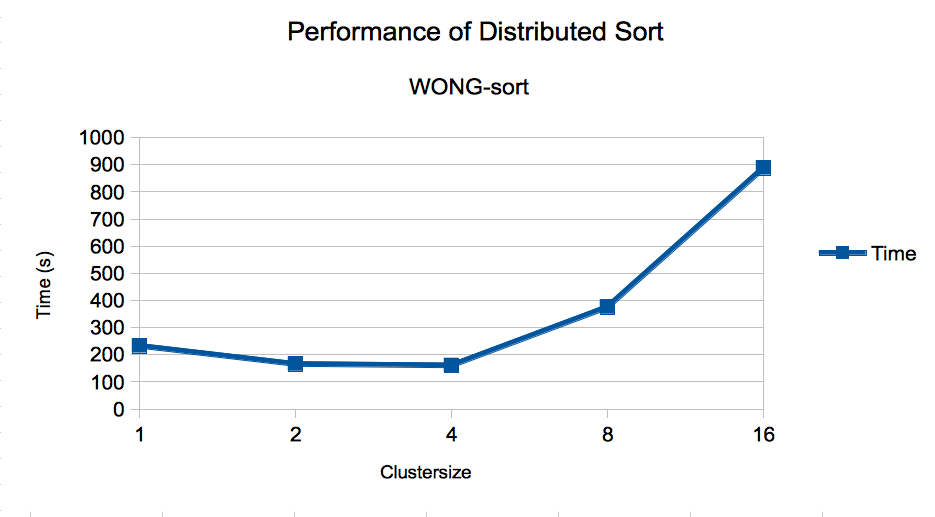
\includegraphics[width=\textwidth]{wong-performance.png}

\par
The slowdown seen here is due to the merging process and it's poor use of both
memory and hard disk locality.  A more efficient merging algorithm and a system for managing I/O over mmap would have significantly improved performance.
In the psort \cite{psort} paper, the authors also use a number of 
optimization techniques including asynchronous I/O and asynchronous network
communication and merging the data.  
\par
Not shown, but also interesting to note is that successive runs of the program
on small data sizes would often vary by upwards of 50\%.  This could be attributed to a number of
factors including network traffic and I/O traffic on both the master and the
slaves.

\begin{thebibliography}{10}
	\bibitem{tam} Nancy Amato, Ravishankar Iyer, Sharad Sundaresan, and Yan Wu. 1998. A Comparison of Parallel Sorting Algorithms on Different Architectures. Technical Report. Texas A \& M University, College Station, TX, USA.
	\bibitem{psort} Paolo Bertasi, Federica Bogo, Marco Bressan, Enoch Peserico. PSORT 2011, pennysort, datamation, joulesort.
	\bibitem{data} Florentina I. Popovici John Bent Brian Forney Andrea Arpaci-Dusseau and Remzi Arpaci-Dusseau. 2001. Datamation 2001: A Sorting Odyssey. University of Madison.
\end{thebibliography}
\end{document}

